%\documentclass[a4paper]{jpconf}
\documentclass{ws-procs9x6} 
\usepackage{graphicx}
\usepackage{amsfonts}
\pagestyle{empty} 
%\documentclass[a4paper]{jpconf}
\begin{document}
\title{New Insight into the Cluster Structure of $^9$Be by Reactions with Deuteron Beam}

\author{S.~M.~Lukyanov$^1$, B.~Urazbekov$^1$, D.~M.~Janseitov$^{2}$, V.~Burjan$^3$, A.~S.~Denikin$^1$, W.~H.~Trzaska$^4$, M.~Harakeh$^5$, D.~Etasse$^6$, T.~Issataev$^{1,7}$, V.~Kroha$^3$, V.~A.~Maslov $^1$, J.~Mrazek$^3$, K.~Mendibayev$^{1,7}$, M.~A.~Naumenko$^1$, I.~Siv\'{a}\v{c}ek$^{1,3}$, V.~Glagolev$^3$, \v{S}.~Pisko\v{r}$^3$, Yu.~E.~Penionzhkevich$^{1,8}$, N.~K.~Skobelev$^1$, I.~Stefan$^9$, D.~Verney$^9$, K.~Kuterbekov$^{7}$ and T.~Zholdybayev$^{10}$}
\address{$^1$ Flerov Laboratory of Nuclear Reactions, JINR, Dubna, Russian Federation} 
\address{$^2$ Bogolyubov Laboratory of Theoretical Physics,JINR, Dubna, Russian Federation}
\address{$^3$ Nuclear Physics Institute, \v{R}e\v{z}, Czech Republic} 
\address{$^4$ Department of Physics, University of Jyv\"askyl\"a, Jyv\"askyl\"a, Finland}
\address{$^5$ KVI-CART, University of Groningen, Groningen, The Netherlands}
\address{$^6$ LPC-Caen, ENSICAEN, Universit\'{e} de Caen, CNRS/IN2P3-ENSI, Caen, France }
\address{$^7$ Eurasian Gumilev University, Astana, Kazakhstan}
\address{$^8$ International University "Dubna", Dubna, 141980, Russian Federation}
\address{$^9$ Institut de Physique Nucl\'{e}aire, Univ. Paris-Sud, Universit\'{e} Paris-Saclay, Orsay, France}
\address{$^{10}$ Nuclear Physicanamcs Institute, Almaty, Kazakhstan}
%\ead{lukyan@jinr.ru}

\begin{abstract}
Angular distributions of protons, deuterons, tritons, and alpha particles emitted in the reaction $^2$H+$^{9}$Be at $E_{lab}$=19.5, 25, and 35~MeV were measured to study the structure of $^9$Be, especially to shed light on the internal clusters and possible cluster transfer of $^5$He. The experiments were performed at sufficiently high energies to ensure suppression of compound nucleus contribution. Thus, the direct reaction mechanism should be mainly responsible for the measured five-nucleon transfer cross section. The analysis suggests a significant contribution of simultaneous five-nucleon transfer in the reaction channel ${^9}$Be($d$,$^4$He)$^7$Li.
\end{abstract}

\keywords{Elastic and inelastic scattering; Transfer reactions; Clusters in light nuclei; Coupled channels; DWBA; Optical model.}

\section{Introduction}
Due to the Borromean structure, special attention has been focused on the $^9$Be nucleus, the breakup of which can proceed directly into two alpha particles and a neutron or via one of two unstable intermediate nuclei such as $^8$Be or $^5$He~\cite{Brown,Papka}.

Scattering of a projectile, such as $^{1,2}$H or $^{3,4}$He, on a target is a standard tool to study the structure of nuclei. This method involves the angular distribution measurement of elastic and inelastic scattering. Energy and angular distributions of the products provide information on the internal structure of the interacting nuclei.

The angular distributions for the $^9$Be($^3$He,$^3$He)$^9$Be, $^9$Be($^3$He,$^5$He)$^7$Be, $^9$Be($^3$He,$^5$Li)$^7$Li, $^9$Be($^3$He,$^6$Be)$^6$He, and $^9$Be($^3$He,$^6$Li)$^6$Li reaction channels were measured and reported in Refs.~\cite{luk1,luk2}. The experimental data were described within the framework of the optical model, the coupled-channel approach and the distorted-wave Born approximation. The performed analysis of the experimental data shows that the potential parameters are quite sensitive to the exit channel and, hence, to the cluster structure of the populated states. The experiment~\cite{luk1,luk2} was an attempt to determine the contribution of the $^8$Be+n and $^5$He+$\alpha$ channels by inclusive measurements. We found that the ratio about 2.7:1 may be assigned to the contributions of these two channels, respectively. That justifies that the $^5$He+$\alpha$ breakup channel plays an important role.

Another motivation was an attempt to find not only the cluster structure (in particular, $^5$He), but also to clarify how the cluster structure is involved into the nuclear reaction mechanism. Indeed, starting from D\'{e}traz~\cite{Detraz1,Detraz2}, multiparticle-multihole structures were expected to occur at rather low excitation energies in nuclei. Four-nucleon transfer reactions are being extensively studied. Despite the complexity of such transfer, one may assume that the nucleons are transferred as a whole, strongly correlated in a cluster with internal quantum numbers of a free particle.

This article is aimed at obtaining new experimental data and their preliminary analysis for the reaction $^2$H+$^{9}$Be at various projectile energies: E$_{lab}$=19.5, 25, and 35 MeV. Compared with the experiment~\cite{Bodek}, the present experiments were performed at sufficiently high energies to ensure suppression of compound nucleus contribution. Thus, the direct reaction mechanism should provide the main contribution to the reaction channels.

\section{Experimental Method}
The experiments were performed using the beam of $^2$H ions on the cyclotron of Nuclear Physics Institute of the Czech Academy of Sciences (\v{R}e\v{z}, Czech Republic), Institut de Physique Nucl\'{e}aire, CNRS-IN2P3, Universit\'{e} Paris-Sud, Universit\'{e} Paris-Saclay, and the Cyclotron facility of the Accelerator Laboratory of the Physics Department of Jyv\"{a}skyl\"{a} University at energies 19.5, 25, and 35 MeV, respectively. The average beam current during the experiment was maintained at 20~nA. The self-supporting Be target was prepared from a thin beryllium foil. To measure (in)elastically scattered ions, a set of four telescopes, each consisting of $\Delta E_0$, $\Delta E$, $E_r$ detectors with thicknesses respectively 12~$\mu$m, 100~$\mu$m, and 3~mm were used. The telescopes were mounted at a distance $\sim$20~cm from the target in the reaction chamber. Particle identification was performed based on the measurements of energy loss $\Delta E$ and residual energy $E_r$, i.e., by the so-called $\Delta E-E$ method.

An example of the two-dimensional plot (yield vs. energy loss $\Delta E$ and residual energy $E_r$) is shown in Fig.~1.
\begin{figure}[htp]
\centering
\includegraphics[width=100mm]{dE_E.eps}
\label{figure}\caption{
Typical particle identification plot for the products of the $^{2}$H+$^9$Be reaction: $p$, $d$, $t$, and $^{4}$He. $\Delta E$ is the energy loss and $E_r$ is the residual energy. Excited states for the $^7$Li reaction channel $^7$Li+$\alpha$ are indicated.}
\label{fig1}
\end{figure}

This experimental technique with good resolution $\sim$150~keV allowed us to identify the particles $p, d, t$, and $^4$He and determine their total deposited energy. The spectra of total deposited energy are shown in Fig.~2. All peaks observed in the histograms in Fig.~2 were identified and found to belong to the ground and the excited states of $^{10}$Be, $^9$Be, $^8$Be, and $^7$Li as the complementary products to the detected particles $p, d, t$, and $^4$He, respectively. That confirms our previous finding about one-step multinucleon transfer and the two body reaction mechanism in the exit reaction channels.
\begin{figure}[htp]
\centering
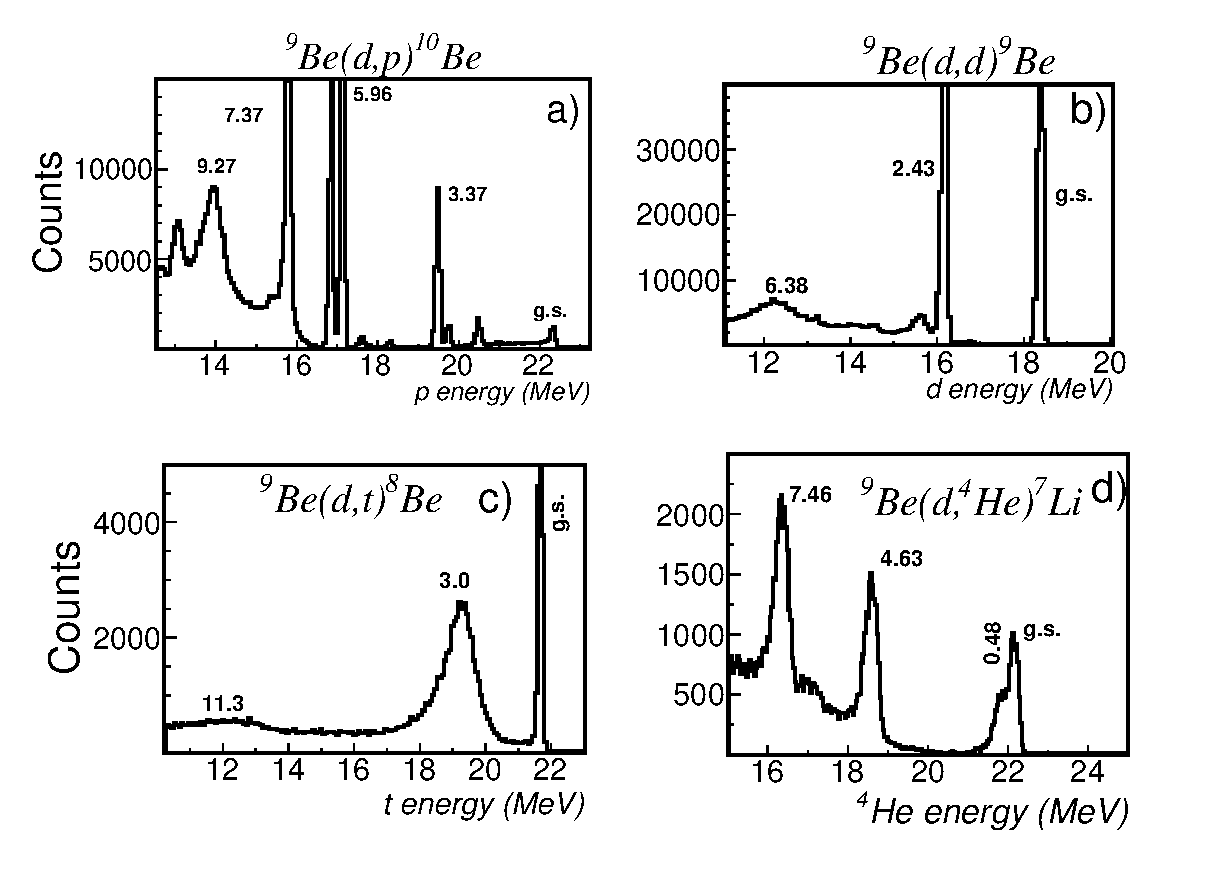
\includegraphics[width=100mm]{d_Etot_Fig2.eps}\\
\label{figure}\caption{Total deposited energy spectra measured at $\theta_{lab}$=32$^\circ$ for the detected $p$ (panel a), $d$ (panel b), $t$(panel c), and $^4$He(panel d). The ground and the excited states of $^7$Li in the case of the detected complementary product $^4$He as well as the ground states and the excited states of $^8$Be, $^9$Be, and $^{10}$Be in the case of the detected complementary products respectively $t, d$, and $p$ were unambiguously identified.}
\label{fig2}
\end{figure}

\section{Results and Data Analysis}
\subsection{Elastic and inelastic scattering}

The differential cross sections for elastic scattering of deuterons on the beryllium target measured at various projectile energies are presented in Fig.~3. The obtained elastic scattering cross sections were analyzed within the optical model available in the NRV web knowledge base on low-energy nuclear physics~\cite{NRV,Denikin}. Theoretical results are shown as the solid curves.
%-----------------------
\begin{figure}[t]
\begin{center}
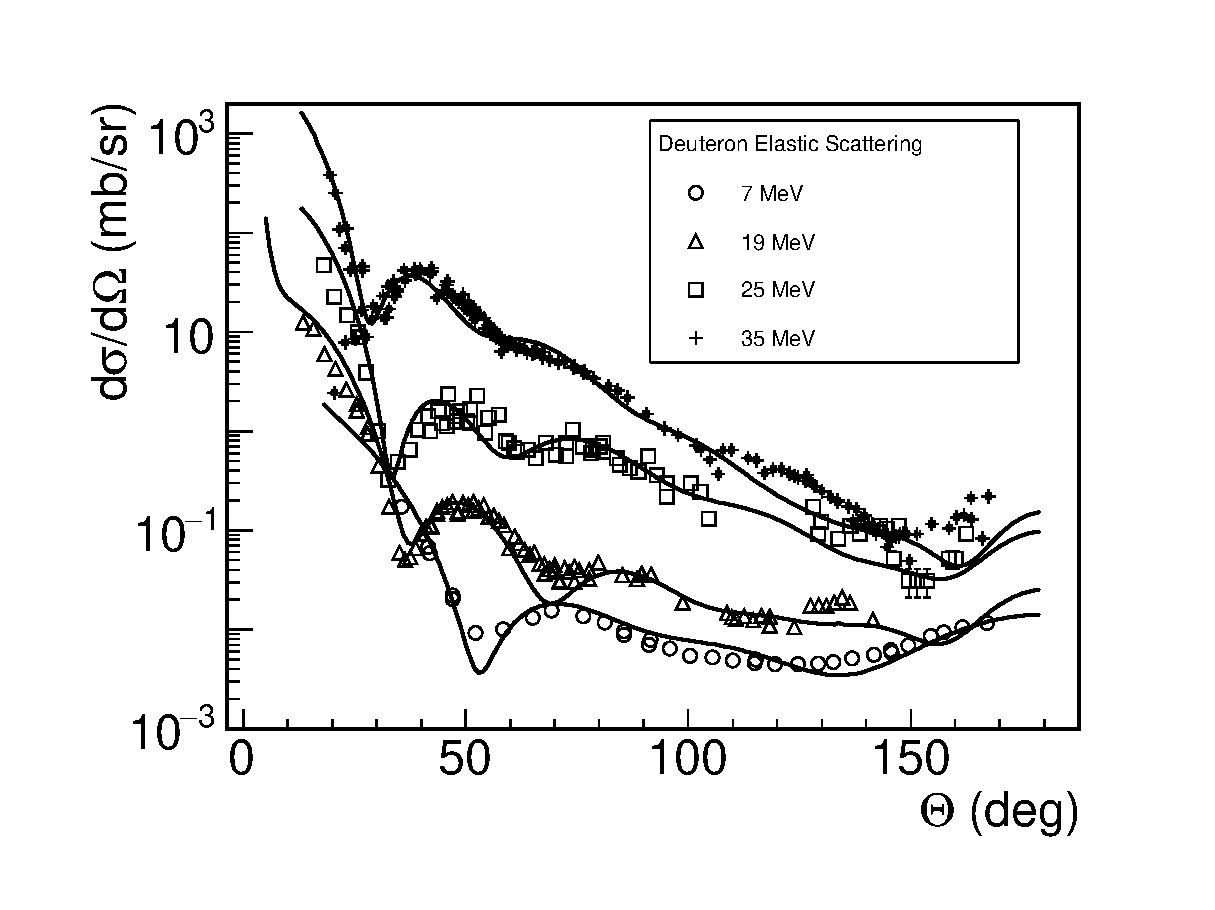
\includegraphics[width=100mm]{d_elastic_factor--lines.eps}\end{center}
\caption{Differential angular distributions for elastic scattering of $d + ^{9}$Be at various projectile energies. Data obtained in the present work at 35, 25, and 19~MeV are shown respectively by ($+$), ($\Box$), and ($\triangle$) symbols; data from~\cite{Bodek} are denoted by ($\circ$) symbols.}
\label{fig3}
\end{figure}
%-----------------------

\subsection{Transfer reaction channels}
Fig.~4a shows experimental angular distributions for $t$+$^8$Be, $^4$He+$^7$Li, and $^4$He+$^7$Li reaction channels as well as the channel leading to the production of boron isotopes. For boron isotopes, only the atomic number $Z$ was identified; we were not able to determine exactly the atomic mass $A$ due to the limitations connected with kinematic broadening and the detector thickness.
%-----------------------
\begin{figure}[htp]
\centering
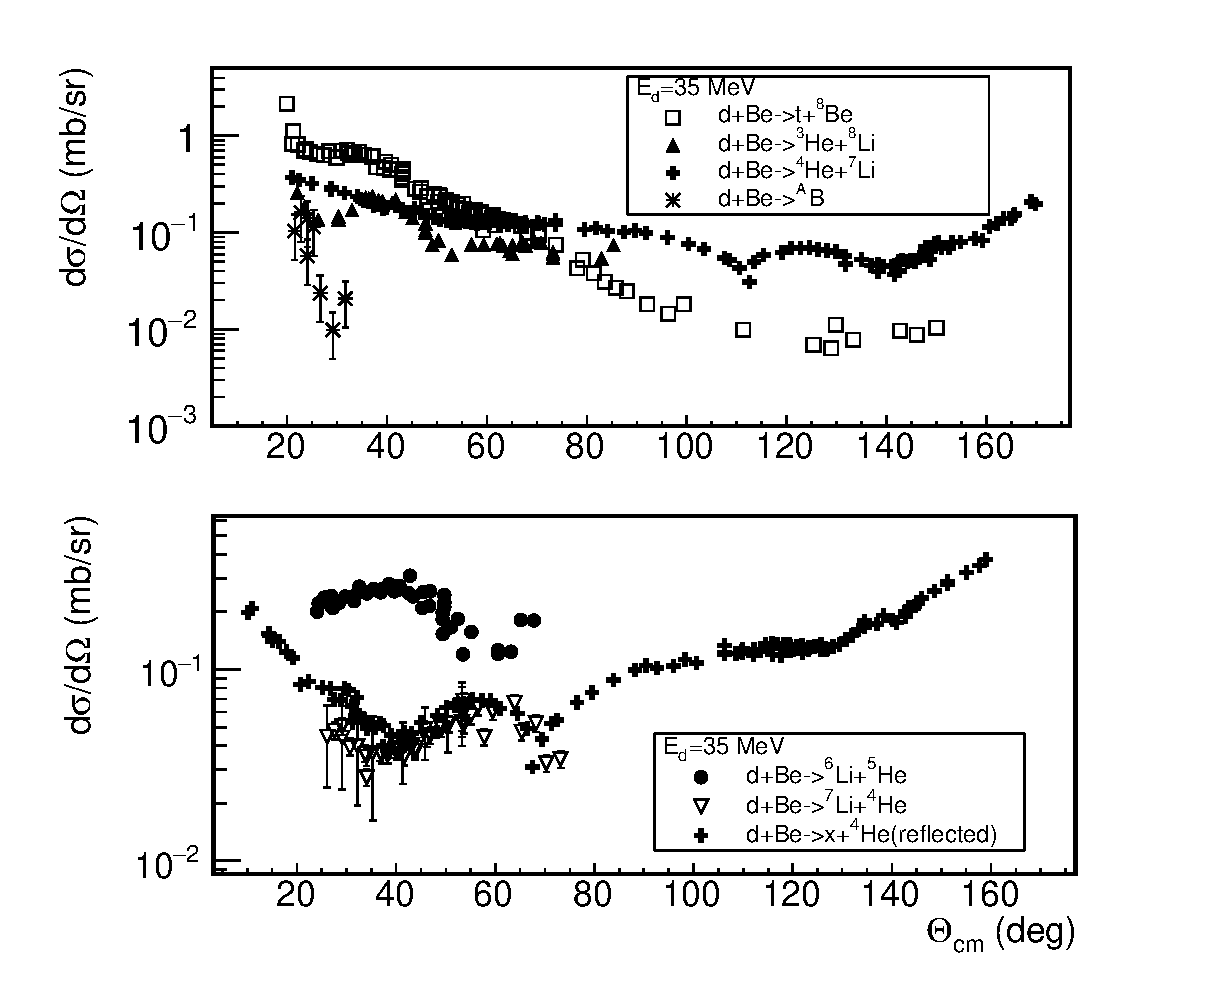
\includegraphics[width=100mm]{p_d_He-transfer-3.eps}
\label{figure}
\caption{a) Experimental angular distributions for $t$+$^8$Be ($\Box$), $^4$He+$^7$Li (${\bf +}$), $^4$He+$^7$Li ($\triangle$) reaction channels. The channel leading to the production of boron isotopes is denoted by ($\ast$).}
\label{fig4}
\end{figure}
%-----------------------

Experimental angular distributions for the detected $^7$Li and $^6$Li are shown in Fig.~4b. Differential angular distribution in the case of the detected $^7$Li as a supplementary product to $^4$He was compared with 90$^{\circ}$-reflected angular distribution for the reaction channel $^4$He+$^7$Li. One may see good overlapping of the differential cross sections for $^7$Li+x and $^4$He+x reaction channels. That confirms the two-body reaction mechanism in exit channel. 

Special attention was paid to the $^4$He+$^7$Li reaction channel which can proceed via two different mechanisms, either by transfer of $d$ (dashed line in Fig.~5) or by transfer of $^5$He (solid line in Fig.~5) from the target to the projectile. In the exit channel both these mechanisms are indistinguishable. However, in the former case, the $^4$He nuclei are expected to fly forward in the center of mass system, whereas in the latter case, they must preferably fly into the backward angles. The calculations carried out within the DWBA method for these two mechanisms at 19 MeV are shown in Fig.~5. Their coherent sum shown as the black curve is in good agreement with the experimental points. It is interesting to note that for the correct description of the magnitude of the data, it is necessary to use sufficiently large values of the spectroscopic factors for the reaction, $S_fS_i = 1.2$. In addition, to describe the structure of the angular distributions, it is also necessary to assume a 30$\%$ admixture of the $d$-state in the structure of $^7$Li. Data analysis for the projectile energy 7 and 35~MeV is in progress.
%-----------------------
\begin{figure}[htp]
\centering
\includegraphics[width=100mm]{fig4_obman.eps}
\label{figure}\caption{Experimental angular distributions for reaction channels $^9$Be($^2$H,$^4$He)$^7$Li ($\bullet$) and $^9$Be($^2$H,$^7$Li)$^4$He ($\circ$) at 19.5~MeV  (for details, see text).}
\label{fig5}
\end{figure}
%-----------------------

Convincing evidence for direct five-nucleon transfer processes has been presented for the first time in the papers~\cite{Bodek,Jarczyk}. Data analysis for these reactions has been usually performed under the assumption of the single-step transfer of the $^5$He cluster. Such an analysis was treated as a proof of the presence of $^5$He clusterization in light nuclei. However, it is possible that five nucleons are transferred not as $^5$He, but most likely via the transfer of an alpha particle and a neutron. Such a mechanism can be quite important because transfer of nucleons as well as alpha particles is known to proceed with large values of the cross sections. The open question is how these particles can be transferred -- simultaneously in a one-step process or sequentially in a two-step process. In Ref.~\cite{Jarczyk}, it was mentioned  that simultaneous transfer is a more general mechanism than transfer of a single five-nucleon cluster because the $\alpha$-particle and the nucleon can change the state of their relative motion during the reaction. Only a specific simultaneous transfer of a nucleon and an $\alpha$ particle, i.e., a correlated transfer, in which the transferred nucleons form the cluster with the quantum numbers of $^5$He, is equivalent to a single five-nucleon cluster transfer.

Our results confirm finding of Refs.~\cite{Bodek,Jarczyk} that the largest contribution corresponds to the transfer of an $\alpha$-particle and a nucleon correlated to $^{5}$He as a whole cluster.

In summary, angular distributions for the $^9$Be($d$,$d$)$^9$Be$^*$, $^9$Be($d$,$p$)$^{10}$Be, $^9$Be($d$,$t$)$^8$Be, and $^9$Be($d$,$^4$He)$^7$Li channels were measured. Experimental angular distributions were described within the optical model, the coupled channel approach, and the distorted wave Born approximation. The optical model provides good agreement with the elastic scattering data. The DWBA calculations agree well with the transfer reaction data. The spectroscopic factors for the systems $^9$Be=$\alpha$+$^5$He and $^7$Li=$d$+$^5$He are close to unity, which confirms the contribution of the considered cluster configurations to the structure of ground states.

The analysis shows that the contribution of the compound nucleus mechanism is negligible. In the ($d$,$^4$He) channel, the deuteron transfer provides only a small contribution, whereas a relatively large contribution of $^5$He transfer is found, in agreement with the result~\cite{Bodek}. This demonstrates that the specific structure of the $^9$Be nucleus as a weakly bound system of two alpha particles and a neutron strongly favors five-nucleon transfer compared to deuteron transfer.

\section*{Acknowledgments}
Authors thank the CANAM project (http://users.canam.ujf.cas.cz) and the mobility grant from the Academy of Finland for providing beam time for the experiments and support. This work was also supported by the Russian Science Foundation, grant No. 17-12-01170.

%\section*{References}
\begin{thebibliography}{8}
\bibitem{Brown}
T~A~D~Brown, P~Papka, B~R~Fulton {\it et al.}, Decay studies for states in $^9$Be up to 11 MeV: Insights into the n+$^{8}$Be and $\alpha+^{5}He$ cluster structure,
{\em Phys. Rev. C} {\bf 76}, 054605 (2007).
\bibitem{Papka}
P~Papka, T~A~D~Brown, B~R~Fulton {\it et al.}, Decay path measurements for the 2.429 MeV state in $^9$B, 
{\em Phys. Rev. C} {\bf 75}, 045803 (2007).
\bibitem{luk1} 
S~M~Lukyanov, A~S~Denikin, E~I~Voskoboynik {\it et al.}, Study of internal structures of $^{9,10}$Be and $^{10}$B in scattering of $^4$He from $^9$Be, 
{\em J. Phys. G} {\bf 41}, 035103 (2014).
\bibitem{luk2}
S~M~Lukyanov, M~Harakeh, M~A~Naumenko {\it et al.}, Some Insights into Cluster Structure of $^9$Be from $^{3}$He+ $^{9}$Be Reaction,
{\em World Journal of Nuclear Science and Technology} {\bf 5} 265 (2015). doi: 10.4236/wjnst.2015.54026.
\bibitem{Detraz1}
C~D\'{e}traz, H~H~Duhm and H~Hafner, The ($^3$He, $^7$Be) Reaction on Light Nuclei,
{\em Nucl. Phys. A} {\bf 147}, 488 (1970).
\bibitem{Detraz2}
C~D\'{e}traz, F~Pougheon, M~Bernas {\it et al.}, Selectivity in the $^{11}$B($^3$He,$^6$Li)$^8$Be reaction,
{\em Nucl. Phys. A} {\bf 228}, 39 (1974).
\bibitem{Bodek}
A~Szczurek, K~Bodek, J~Krug {\it et al.}, Mechanism of Reactions Induced by 7 MeV Deuterons on $^9$Be[(d, p), (d, d), (d, t), (d, $^4$He)],
{\em Zeitschrift f{\"u}r Physik A Atomic Nuclei}, {\bf 333}, 271 (1989).
\bibitem{FRESCO}
http://www.ianthompson.org/surrey and http://nrv.jinr.ru
\bibitem{NRV}
V.I. Zagrebaev, A.S. Denikin and A.P. Alekseev, {\em http://nrv.jinr.ru/nrv/ "Optical model of elastic scattering"}.
\bibitem{Denikin}
A. Denikin, S. Lukyanov, S.Khlebnikov {\it et al.}, Inelastic scattering and clusters transfer in $^{3,4}$He + $^9$Be reactions, 
 {\em Physics of Particles and Nuclei Letters}, 2015, Vol. {\bf 12}, No. 5, pp. 703–712. Pleiades Publishing, Ltd., 2015.
\bibitem{Jarczyk}
L. Jarczyk, B. Kamys, M. Kistryn {\it et al.}, Five-Nucleon Simultaneous and Sequential Transfer in the $^{12}$C($^{11}$B, $^6$Li)$^{17}$O and $^{12}$C(d, $^7$Li)$^7$Be Reactions, {\em Phys. Rev. C} {\bf 54},v.3, 1302 (1996).
\bibitem{Kamus}
B. Kamys, Z. Rudy, J. Kisiel, E. Kwasniewicz {\it et al.}, Simultaneous and Sequential Transfer of Proton and Alpha-Particle in Elastic $^{11}$B + $^{16}$O Scattering, 
{\em Zeitschrift f{\"u}r Physik A Atomic Nuclei}, {\bf 342}, 149 (1992).
\end{thebibliography}






\end{document}


